\section{Resultados}
\subsection{Comparação de eficiencia}
Cada kernel foi executado 3000 vezes em sequência. A GPU tem um mecânismo que faz um cache do código do kernel e também
da memória que ele utiliza, então podemos desconsiderar a comunicação da CPU com a GPU neste caso, deixando os nossos resultados 
mais próximos do tempo de execução dos kernels.

É importante levar em conta que a GPU não estava rodando somente o kernel, já que os drivers necessários para a execução 
do mesmo estão atrelados ao X Window System, então o kernel sofreu interrupções na GPU, para que a interface gráfica do 
Ubuntu fosse renderizada.

\subsubsection{Kernel memory-bound}
Os resultados dos kernels memory-bound:

\begin{figure}[H]
  \begin{center}
    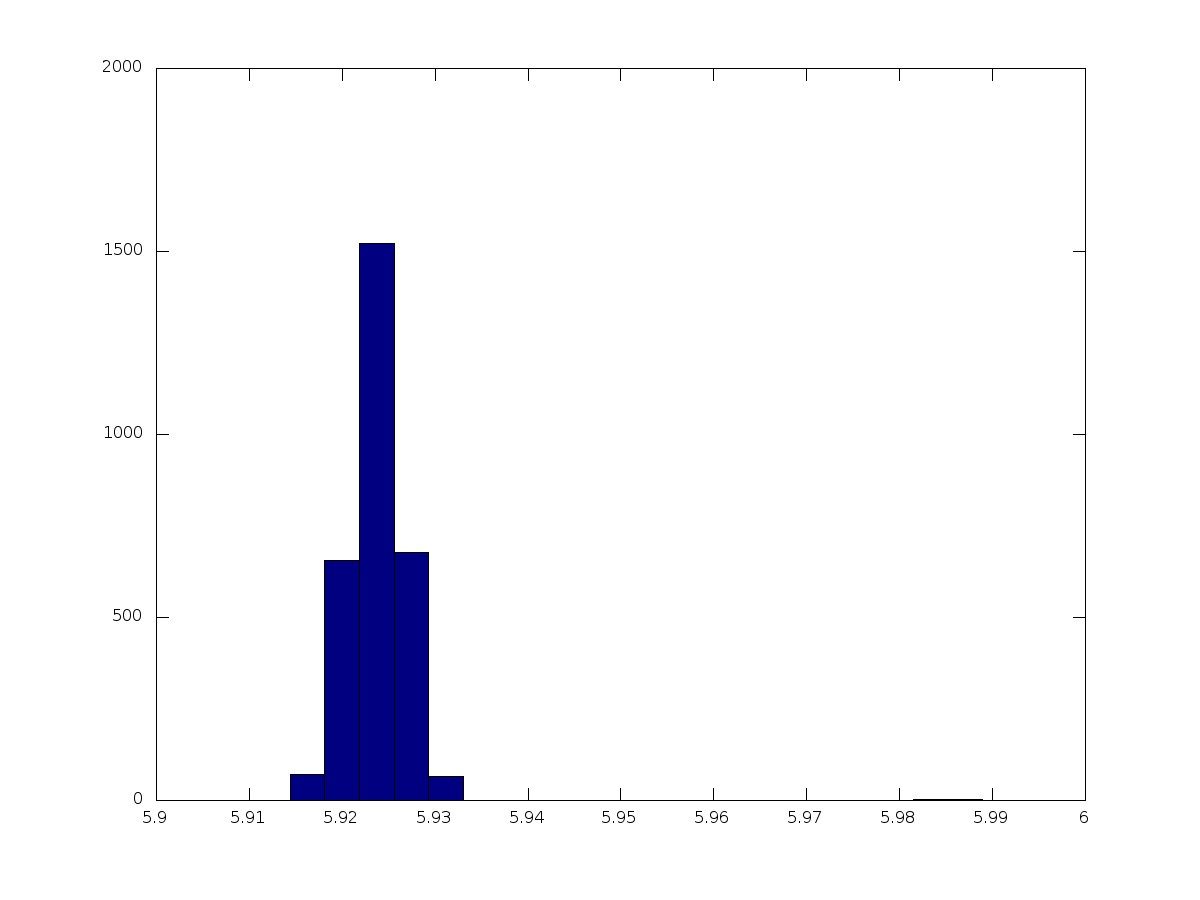
\includegraphics[scale=0.3]{resultados_cuda_memory_histo.jpg}
    \label{fig:Kernel Memory-Bound CUDA}
    \caption{Kernel Memory-Bound CUDA}
  \end{center}
\end{figure}

\begin{figure}[H]
  \begin{center}
    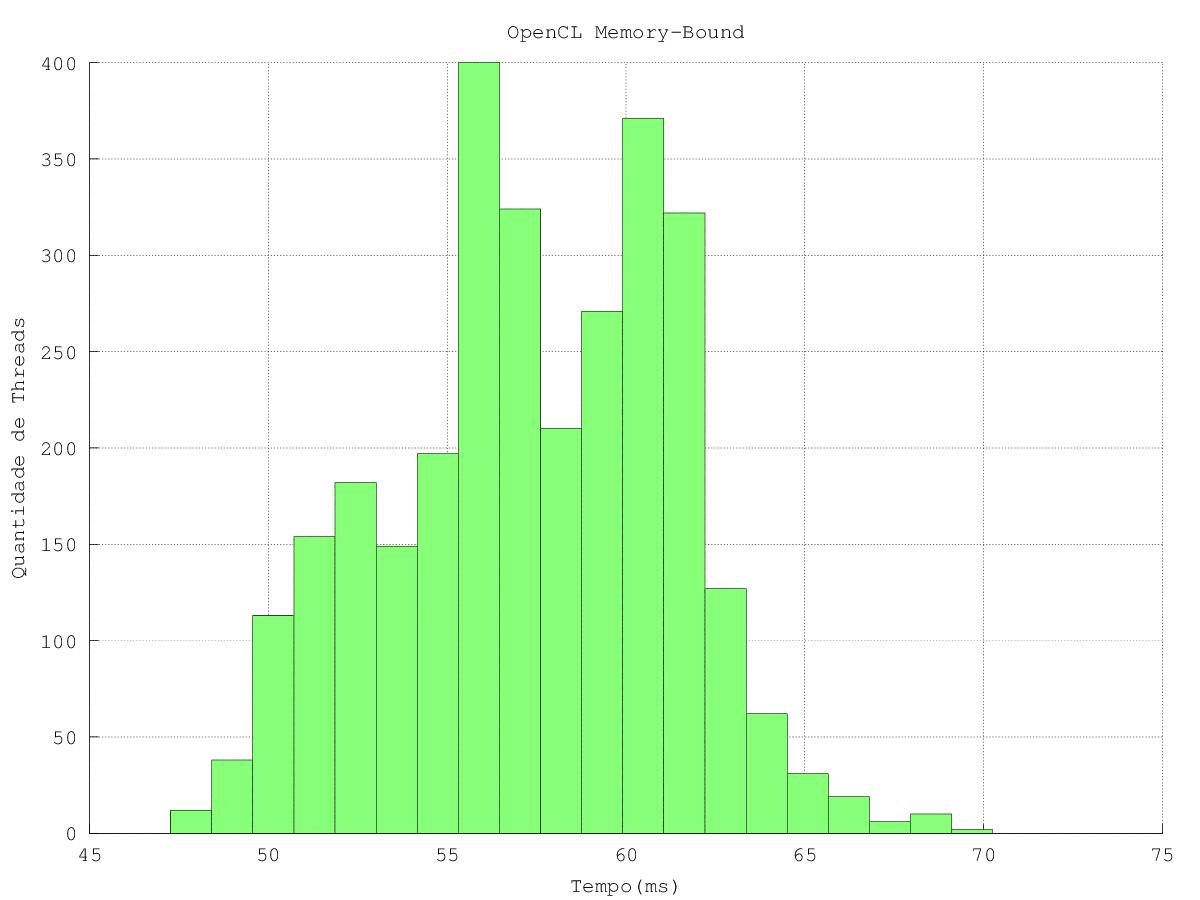
\includegraphics[scale=0.3]{resultados_opencl_memory_histo.jpg}
    \label{fig:Kernel Memory-Bound OpenCL}
    \caption{Kernel Memory-Bound OpenCL}
  \end{center}
\end{figure}

\subsubsection{Kernel processing-bound}

\begin{figure}[H]
  \begin{center}
    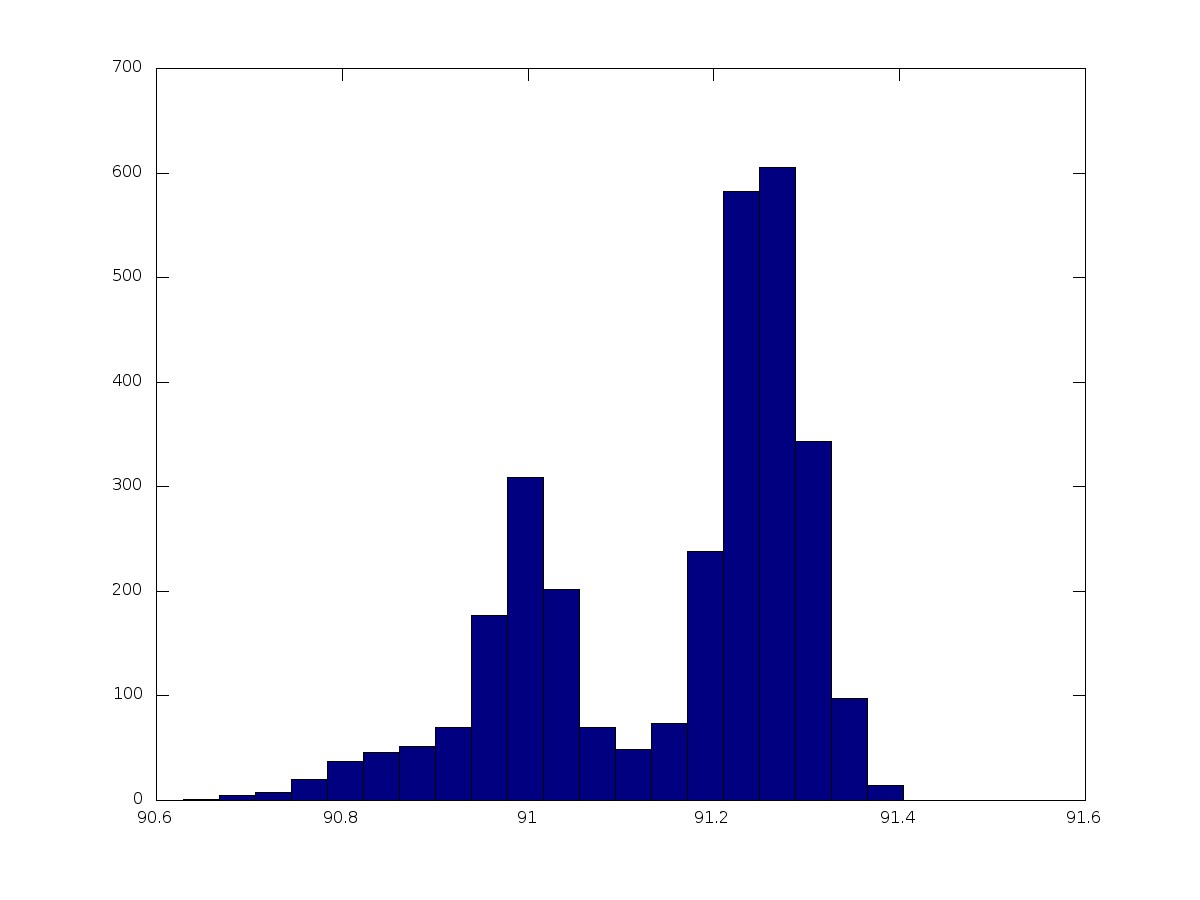
\includegraphics[scale=0.3]{resultados_cuda_process_histo.jpg}
    \label{fig:Kernel Memory-Bound CUDA}
    \caption{Kernel Memory-Bound CUDA}
  \end{center}
\end{figure}

\begin{figure}[H]
  \begin{center}
    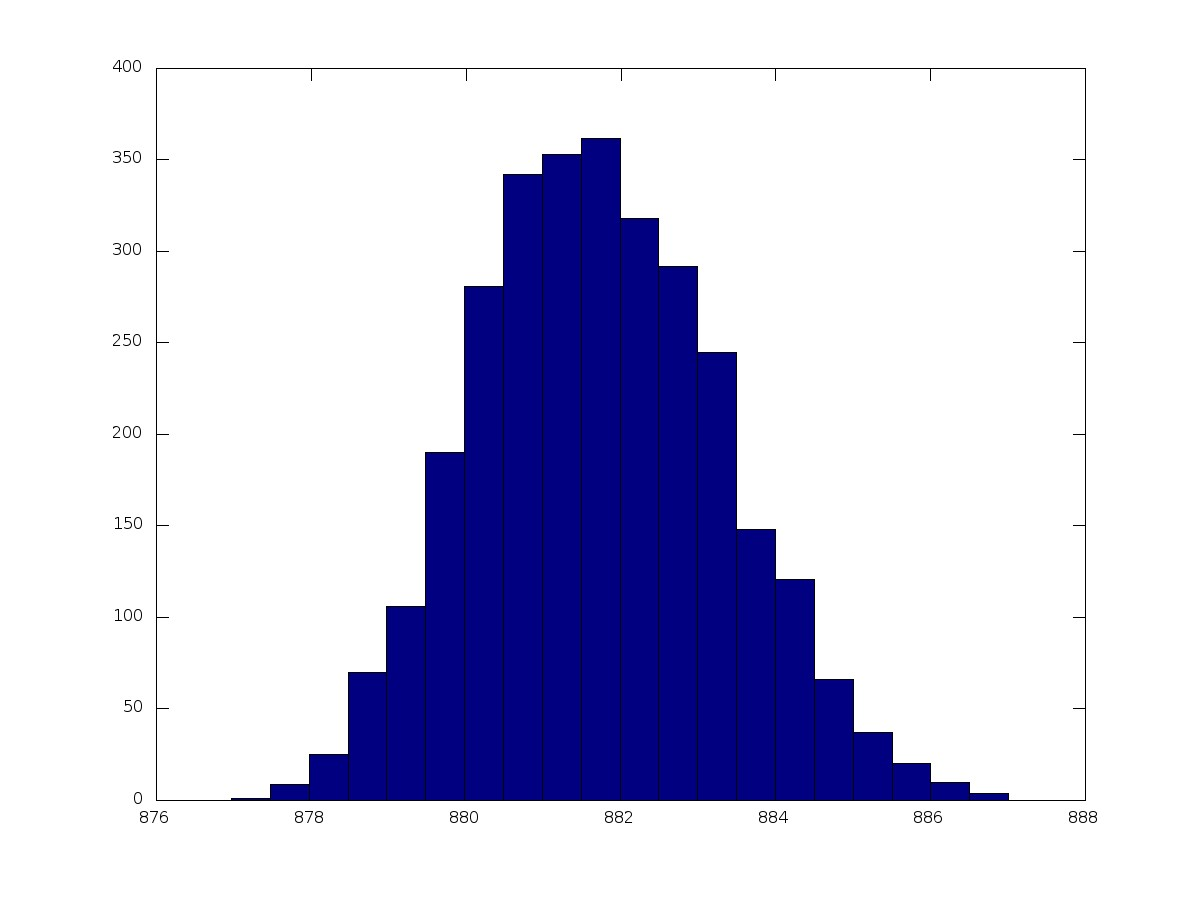
\includegraphics[scale=0.3]{resultados_opencl_process_histo.jpg}
    \label{fig:Kernel Memory-Bound OpenCL}
    \caption{Kernel Memory-Bound OpenCL}
  \end{center}
\end{figure}

\subsection{Comparação dos .ptx}

Vamos analisar os .ptx resultantes dos kernels de cópia das matrizes:

O kernel do OpenCL: 

\begin{lstlisting}
  .version 3.0
  .target sm_21, texmode_independent
  .address_size 32


  .entry matrixcopy(
	    .param .u32 .ptr .global .align 4 matrixmulti_param_0,
	    .param .u32 .ptr .global .align 4 matrixmulti_param_1,
	    .param .u32 .ptr .global .align 4 matrixmulti_param_2,
	    .param .u32 .ptr .global .align 4 matrixmulti_param_3
    )
    {
	    .reg .f32 	%f<2>;
	    .reg .s32 	%r<21>;


	    ld.param.u32 	%r9, [matrixmulti_param_0];
	    ld.param.u32 	%r10, [matrixmulti_param_1];
	    ld.param.u32 	%r11, [matrixmulti_param_2];
	    mov.u32 	%r1, %envreg3;
	    mov.u32 	%r2, %ntid.x;
	    mov.u32 	%r3, %ctaid.x;
	    mov.u32 	%r4, %tid.x;
	    add.s32 	%r12, %r4, %r1;
	    mad.lo.s32 	%r13, %r3, %r2, %r12;
	    mov.u32 	%r5, %envreg4;
	    mov.u32 	%r6, %ntid.y;
	    mov.u32 	%r7, %ctaid.y;
	    mov.u32 	%r8, %tid.y;
	    add.s32 	%r14, %r8, %r5;
	    mad.lo.s32 	%r15, %r7, %r6, %r14;
	    ld.global.u32 	%r16, [%r11];
	    mad.lo.s32 	%r17, %r15, %r16, %r13;
	    shl.b32 	%r18, %r17, 2;
	    add.s32 	%r19, %r9, %r18;
	    add.s32 	%r20, %r10, %r18;
	    ld.global.f32 	%f1, [%r19];
	    st.global.f32 	[%r20], %f1;
	    ret;
    }
\end{lstlisting}

E o do CUDA:

\begin{lstlisting}
  .version 3.0
  .target sm_20
  .address_size 64

	  .file	1 "/tmp/tmpxft_00003b7f_00000000-9_memory.cpp3.i"
	  .file	2 "memory.cu"

  .entry _Z10MatrixCopyPfS_ii(
	    .param .u64 _Z10MatrixCopyPfS_ii_param_0,
	    .param .u64 _Z10MatrixCopyPfS_ii_param_1,
	    .param .u32 _Z10MatrixCopyPfS_ii_param_2,
	    .param .u32 _Z10MatrixCopyPfS_ii_param_3
    )
    {
	    .reg .f32 	%f<2>;
	    .reg .s32 	%r<13>;
	    .reg .s64 	%rl<8>;


	    ld.param.u64 	%rl1, [_Z10MatrixCopyPfS_ii_param_0];
	    ld.param.u64 	%rl2, [_Z10MatrixCopyPfS_ii_param_1];
	    ld.param.u32 	%r1, [_Z10MatrixCopyPfS_ii_param_3];
	    cvta.to.global.u64 	%rl3, %rl2;
	    mov.u32 	%r2, %ntid.x;
	    mov.u32 	%r3, %ctaid.x;
	    mov.u32 	%r4, %tid.x;
	    mad.lo.s32 	%r5, %r2, %r3, %r4;
	    mov.u32 	%r6, %ntid.y;
	    mov.u32 	%r7, %ctaid.y;
	    mov.u32 	%r8, %tid.y;
	    mad.lo.s32 	%r9, %r6, %r7, %r8;
	    mad.lo.s32 	%r10, %r9, %r1, %r5;
	    cvta.to.global.u64 	%rl4, %rl1;
	    mul.wide.s32 	%rl5, %r10, 4;
	    add.s64 	%rl6, %rl4, %rl5;
	    add.s64 	%rl7, %rl3, %rl5;
	    ld.global.f32 	%f1, [%rl6];
	    st.global.f32 	[%rl7], %f1;
	    ret;
    }
\end{lstlisting}

A primeira diferença entre os .ptx está na configuração da máquina PTX. O OpenCL configura a Compute Capability para 2.1, enquanto
o CUDA configura para 2.0. A configuração do CUDA foi feita via compilação usando a flag \textit{-arch=compute\_20}, enquanto a do
OpenCL foi automática. O OpenCL ainda define, por padrão, o método que ele usa para manipular texturas, com o parâmetro 
\textit{texmode\_independent} da diretiva \textit{.target}. O CUDA trabalha com endereçamento de 64 bits enquanto o OpenCL com de
32 bits.

Na declaração dos parâmetros, o OpenCL os define como ponteiros para a memória global e define o alinhamento em bytes da memória
através do \textit{.align N}, N sendo o número de bytes. Como foi dito anteriormente, o CUDA não define para qual tipo de memória
os ponteiros apontarão, provavelmente para deixar que o PTX decida isso e otimize o acesso a memória, então é necessário
transformar os ponteiros de genéricos para globais.

O CUDA e o OpenCL usam o mesmo número de registradores, mas o CUDA usa 8 registradores de tamanho extendido ( \textbf{.reg .s64 \%rl<8>} )
para computações com os parâmetros.

Ao calcular o índice global de uma thread, o OpenCL usa um registrador a mais que o CUDA, o \textit{envreg}. A documentação do
PTX define esse registrador como um registrador \textit{read-only} com conteúdo definido pelo driver. Não existe nada falando sobre
o conteúdo desse registrador tanto na documentação do OpenCL como na do PTX, mas dado que ele é somado ao ao índice de uma thread
dentro de um bloco e o CUDA não permita indexação com um offset, esse registrador deve conter o offset dos índices dos
\textit{work-item} do OpenCL.

O resto do kernel é praticamente igual, a menos do endereçamento ( novamente, o CUDA usa 64 bits enquanto o OpenCL 32 ) e o fato
do OpenCL optar por uma instrução shift left para multiplicar um número por 4 enquanto o CUDA usa uma instrução de multiplicação. \\

Agora vamos analizar os .ptx resultantes da compilação dos kernels de multiplicação de matrizes.

O .ptx do OpenCL:

\begin{lstlisting}
   .version 3.0
  .target sm_21, texmode_independent
  .address_size 32


  .entry matrixmulti(
	    .param .u32 .ptr .global .align 4 matrixmulti_param_0,
	    .param .u32 .ptr .global .align 4 matrixmulti_param_1,
	    .param .u32 .ptr .global .align 4 matrixmulti_param_2,
	    .param .u32 .ptr .global .align 4 matrixmulti_param_3
    )
    {
	    .reg .f32 	%f<5>;
	    .reg .pred 	%p<3>;
	    .reg .s32 	%r<43>;


	    ld.param.u32 	%r3, [matrixmulti_param_2];
	    ld.param.u32 	%r4, [matrixmulti_param_3];
	    mov.u32 	%r12, %envreg3;
	    mov.u32 	%r13, %ntid.x;
	    mov.u32 	%r14, %ctaid.x;
	    mov.u32 	%r15, %tid.x;
	    add.s32 	%r20, %r15, %r12;
	    mad.lo.s32 	%r5, %r14, %r13, %r20;
	    mov.u32 	%r16, %envreg4;
	    mov.u32 	%r17, %ntid.y;
	    mov.u32 	%r18, %ctaid.y;
	    mov.u32 	%r19, %tid.y;
	    add.s32 	%r21, %r19, %r16;
	    mad.lo.s32 	%r6, %r18, %r17, %r21;
	    ld.global.u32 	%r22, [%r4];
	    mad.lo.s32 	%r23, %r22, %r5, %r6;
	    shl.b32 	%r24, %r23, 2;
	    add.s32 	%r25, %r3, %r24;
	    mov.u32 	%r26, 0;
	    st.global.u32 	[%r25], %r26;
	    ld.global.u32 	%r41, [%r4];
	    setp.eq.s32 	%p1, %r41, 0;
	    @%p1 bra 	BB0_3;

	    mov.u32 	%r42, 0;

    BB0_2:
	    mad.lo.s32 	%r28, %r41, %r5, %r42;
	    shl.b32 	%r29, %r28, 2;
	    ld.param.u32 	%r37, [matrixmulti_param_0];
	    add.s32 	%r30, %r37, %r29;
	    mad.lo.s32 	%r31, %r41, %r42, %r6;
	    shl.b32 	%r32, %r31, 2;
	    ld.param.u32 	%r38, [matrixmulti_param_1];
	    add.s32 	%r33, %r38, %r32;
	    ld.global.f32 	%f1, [%r33];
	    ld.global.f32 	%f2, [%r30];
	    mad.lo.s32 	%r34, %r41, %r5, %r6;
	    shl.b32 	%r35, %r34, 2;
	    ld.param.u32 	%r39, [matrixmulti_param_2];
	    add.s32 	%r36, %r39, %r35;
	    ld.global.f32 	%f3, [%r36];
	    fma.rn.f32 	%f4, %f2, %f1, %f3;
	    st.global.f32 	[%r36], %f4;
	    ld.param.u32 	%r40, [matrixmulti_param_3];
	    ld.global.u32 	%r41, [%r40];
	    add.s32 	%r42, %r42, 1;
	    setp.lt.u32 	%p2, %r42, %r41;
	    @%p2 bra 	BB0_2;

    BB0_3:
	    ret;
    }
\end{lstlisting}

E o .ptx do CUDA:

\begin{lstlisting}
  .version 3.0
  .target sm_20
  .address_size 64

	  .file	1 "/tmp/tmpxft_00001760_00000000-9_process.cpp3.i"
	  .file	2 "process.cu"

  .entry _Z10MatrixMultiPfS_S_i(
	    .param .u64 _Z10MatrixMultiPfS_S_i_param_0,
	    .param .u64 _Z10MatrixMultiPfS_S_i_param_1,
	    .param .u64 _Z10MatrixMultiPfS_S_i_param_2,
	    .param .u32 _Z10MatrixMultiPfS_S_i_param_3
    )
    {
	    .reg .f32 	%f<7>;
	    .reg .pred 	%p<3>;
	    .reg .s32 	%r<31>;
	    .reg .s64 	%rl<20>;


	    ld.param.u64 	%rl11, [_Z10MatrixMultiPfS_S_i_param_0];
	    ld.param.u64 	%rl12, [_Z10MatrixMultiPfS_S_i_param_1];
	    ld.param.u64 	%rl13, [_Z10MatrixMultiPfS_S_i_param_2];
	    ld.param.u32 	%r1, [_Z10MatrixMultiPfS_S_i_param_3];
	    cvta.to.global.u64 	%rl1, %rl12;
	    cvta.to.global.u64 	%rl2, %rl11;
	    mov.u32 	%r2, %ntid.x;
	    mov.u32 	%r3, %ctaid.x;
	    mov.u32 	%r4, %tid.x;
	    mad.lo.s32 	%r10, %r2, %r3, %r4;
	    mov.u32 	%r5, %ntid.y;
	    mov.u32 	%r6, %ctaid.y;
	    mov.u32 	%r7, %tid.y;
	    mad.lo.s32 	%r11, %r5, %r6, %r7;
	    mad.lo.s32 	%r12, %r11, %r1, %r10;
	    cvta.to.global.u64 	%rl14, %rl13;
	    mul.wide.s32 	%rl15, %r12, 4;
	    add.s64 	%rl3, %rl14, %rl15;
	    mov.u32 	%r30, 0;
	    st.global.u32 	[%rl3], %r30;
	    setp.lt.s32 	%p1, %r1, 1;
	    @%p1 bra 	BB0_3;

	    mul.wide.s32 	%rl16, %r10, 4;
	    add.s64 	%rl19, %rl1, %rl16;
	    ld.param.u32 	%r23, [_Z10MatrixMultiPfS_S_i_param_3];
	    mul.wide.s32 	%rl5, %r23, 4;
	    mul.lo.s32 	%r18, %r23, %r11;
	    mul.wide.s32 	%rl17, %r18, 4;
	    add.s64 	%rl18, %rl2, %rl17;
	    mov.f32 	%f6, 0f00000000;

    BB0_2:
	    ld.global.f32 	%f4, [%rl19];
	    ld.global.f32 	%f5, [%rl18];
	    fma.rn.f32 	%f6, %f5, %f4, %f6;
	    st.global.f32 	[%rl3], %f6;
	    add.s64 	%rl19, %rl19, %rl5;
	    add.s64 	%rl18, %rl18, 4;
	    add.s32 	%r30, %r30, 1;
	    ld.param.u32 	%r22, [_Z10MatrixMultiPfS_S_i_param_3];
	    setp.lt.s32 	%p2, %r30, %r22;
	    @%p2 bra 	BB0_2;

    BB0_3:
	    ret;
    }
\end{lstlisting}

Os dois .ptx ainda dividem as mesmas diferenças e semelhanças que os anteriores até o cálculo dos índices. Após calcular os índices,
eles atribuem o valor 0 para a variável $k$, que será usada pelo loop que calcula o resultado da multiplicação das duas matrizes
passadas para uma posição da matriz resultante. Aqui já vemos como os registradores lógicos e o símbolo $@$ são usados para
controlar o fluxo dentro da linguagem PTX.

Esse kernel introduz uma instrução que ainda não foi apresentada, a \textit{fma}. Ela faz a mesma coisa que a \textit{mad} mas para
floats, ou seja, ela multiplica o segundo parâmetro no terceiro, soma isso no quarto e guarda o resultado no primeiro. Ela garante
que não ocorre perda de precisão.
